\documentclass[11pt,a4paper,oneside]{report}

% Encodage et langue
\usepackage[utf8]{inputenc}
\usepackage[T1]{fontenc}
\usepackage[french]{babel}

% Polices modernes
\usepackage{lmodern}
\usepackage{mathpazo} % Utilisation de Palatino pour une apparence élégante
\linespread{1.05} % Augmenter légèrement l'interligne pour améliorer la lisibilité

% Mathématiques et graphiques
\usepackage{amsmath}
\usepackage{graphicx}
\usepackage{float}
\usepackage{tikz}

% Mise en page
\usepackage{geometry}
\geometry{left=2.0cm,right=2.0cm,top=2.0cm,bottom=2.0cm}

% En-têtes et pieds de page
\usepackage{fancyhdr}
\pagestyle{fancy}
\fancyhf{}
\renewcommand{\chaptermark}[1]{\markboth{#1}{}}
\rhead{\leftmark}
\cfoot{\thepage}
\renewcommand{\headrulewidth}{0.4pt}
\renewcommand{\footrulewidth}{0.4pt}

% Pour les pages spécifiques sans header et footer
\fancypagestyle{plain}{
    \fancyhf{}
    \renewcommand{\headrulewidth}{0pt}
    \renewcommand{\footrulewidth}{0pt}
}

% Titres
\title{Rapport ArchiLogicielle}
\author{Paul Perigault / Owen Rebeller}
\date{Mai 2024}

% Listes de code
\usepackage{listings}
\usepackage{xcolor}
\lstdefinestyle{mystyle}{
    backgroundcolor=\color{lightgray!20},
    commentstyle=\color{green},
    keywordstyle=\color{blue},
    numberstyle=\tiny\color{gray},
    stringstyle=\color{red},
    basicstyle=\ttfamily,
    inputencoding=utf8,
    extendedchars=false,
    breakatwhitespace=false,
    breaklines=true,
    captionpos=b,
    keepspaces=true,
    numbers=left,
    numbersep=5pt,
    showspaces=false,
    showstringspaces=false,
    showtabs=false,
    tabsize=2,
    literate= {á}{{\'a}}1
        {é}{{\'e}}1
        {í}{{\'i}}1
        {ó}{{\'o}}1
        {ú}{{\'u}}1
        {ê}{{\^e}}1
        {è}{{\`e}}1
}
\lstset{style=mystyle}

% Hyperliens
\usepackage[pdfborder={0 0 0}]{hyperref}

% Tableaux
\usepackage{array, tabularx, longtable, booktabs}

% Références
\usepackage{apalike}

% Table des matières et autres
\usepackage{minitoc}
\usepackage{enumitem}
\usepackage{epigraph}
\usepackage{lscape}
\usepackage{mdframed}
\mdfdefinestyle{summary}{
    innertopmargin=10pt,
    innerbottommargin=10pt,
    innerleftmargin=10pt,
    innerrightmargin=10pt,
    backgroundcolor=gray!10,
    linecolor=gray!50,
    linewidth=1pt,
    frametitleaboveskip=\dimexpr-\ht\strutbox\relax
}
\usepackage{emptypage}
\usepackage{multicol}
\usepackage{subcaption}

% Captions configuration
\usepackage{caption}
\captionsetup{font={sf, sl, small}, margin=3mm}
\captionsetup[lstlisting]{singlelinecheck=false}

% Personnalisation des sections et table des matières
\usepackage{titlesec}
\usepackage{tocloft}
\usepackage{sectsty}
\usepackage{flags}

% Couleurs personnalisées
\definecolor{chaptercolor}{RGB}{0, 102, 204}
\definecolor{subsectioncolor}{RGB}{0, 153, 51}
\definecolor{sectioncolor}{RGB}{204, 0, 102}

\chapterfont{\color{chaptercolor}}
\sectionfont{\color{sectioncolor}}
\subsectionfont{\color{subsectioncolor}}

% Table des matières personnalisée
\renewcommand{\cftsecfont}{\color{sectioncolor}}
\renewcommand{\cftsubsecfont}{\color{subsectioncolor}}
\renewcommand{\cftsecpagefont}{\color{sectioncolor}}
\renewcommand{\cftsubsecpagefont}{\color{subsectioncolor}}
\setlength{\cftbeforesecskip}{0pt}
\setlength{\cftbeforesubsecskip}{0pt}
\setlength{\cftaftertoctitleskip}{10pt} % Réduire l'espacement après le titre de la table des matières
\setlength{\cftbeforetoctitleskip}{10pt} % Réduire l'espacement avant le titre de la table des matières

% Optimisation
\newcommand{\anneeUniversitaire}{2023/2024}
\newcommand{\prenomNOM}{Perigault Paul - Rebeller Owen}
\newcommand{\dateCreation}{09/06/2024}
\newcommand{\sujetMission}{R4.01}

% Hauteur de l'en-tête
\setlength{\headheight}{15pt}

\begin{document}

    % Page de titre sans header/footer
    \thispagestyle{plain}
    
\begin{titlepage}

    \newcommand{\HRule}{\rule{\linewidth}{0.5mm}} % épaisseur de lignes horizontales
    \setlength\fboxrule{2pt} % épaisseur de la boîte de mission

    \begin{center}
        % Logos et année universitaire
        \vspace*{2cm} % Espace avant le logo
        
\includegraphics[width=10cm]{title/iutLogo}
        \vskip 3em % Espace après le logo
        \fontsize{15}{}\textbf{\anneeUniversitaire}

        % Titre principal
        \vskip 1em
        \Huge\textbf{RAPPORT ARCHI LOGICIELLE}
        \vskip 1em
        \Large présenté par
        \vskip 1em
        \fontsize{20}{}\textbf{\prenomNOM}

        \vskip 0.2em
        \Large (210) - (208)

        % Détails de la mission
        \vskip 2em
        \Large Fait le \dateCreation

        % Sujet de la mission
        \vskip 2em
        \Large Ressource :
        \vskip 0.5em
        \fbox{
            \begin{minipage}[c][3em]{0.9\textwidth}
                \centering
                \Large\textbf{\sujetMission}
            \end{minipage}
        }

        % Ligne horizontale
        \vskip 1em
        \HRule
    \end{center}

    \vfill % remplit le reste de la page avec des espaces

\end{titlepage}


    % Résumé sans header/footer
    \clearpage
    \thispagestyle{plain}

    % Remerciements sans header/footer
    \clearpage
    \thispagestyle{plain}

    % Table des matières
    \clearpage
    \tableofcontents
    \clearpage

    % Sections principales
    \pagestyle{fancy} % Appliquer l'en-tête personnalisé à partir de ce point
    \chapter{Côté Serveur}


\section{Structuration du code}

Pour notre architecture nous avons structuré le code en trois parties : le client, la configuration et le serveur.

\begin{itemize}
    \item \textbf{Client} : Il gère la communication avec le serveur. Il a aussi son propre \textit{main}.
    \item \textbf{Configuration} : Il contient la classe \textit{Config.java} et le fichier \textit{config.json} pour la configuration des paramètres de l'application. Ce sont les bonnes pratiques de sécurité qui nous ont poussés à faire ceci.
    \item \textbf{Serveur} : Il comprend différents sous-modules :
    \begin{itemize}
        \item \textbf{Base de données} : Ce module gère la connexion à la base de données ainsi que les opérations sur cette dernière.
        \item \textbf{Éléments} : Défini les entités de l’application telles qu’un \textit{Document} et un \textit{Abonne}.
        \item \textbf{Exceptions} : Gère les différentes exceptions spécifiques à l’application.
        \item \textbf{Opérations} : Regroupe les différents services de l’application (Réservation, Emprunt, Retour).
        \item \textbf{Serveur} : Implémente le protocole de communication utilisé par l’application.
        \item \textbf{Utilitaire} : Fournit des méthodes utiles à l’application et donc réutilisables.
        \item \textbf{TimerTask} : Ce module permet de gérer les tâches planifiées.
    \end{itemize}
    Le serveur a aussi son propre \textit{main} afin d'être exécuté indépendamment du client.
\end{itemize}


\section{Code Stable}

Pour ce projet, nous avons mis en place plusieurs dispositifs pour rendre le code maintenable et stable.

Premièrement, nous avons utilisé des \textcolor{red}{factories} pour faciliter la création d'éléments en grande quantité. Nous avons implémenté une factory dédiée aux serveurs ce qui nous permet de générer autant de serveurs que nécessaire. Cela nous offre la flexibilité de remplacer ou mettre à jour un serveur sans affecter le reste du code.

Une factory pour les données a été mise en place pour charger les données depuis la base de données lors de l’initialisation de l’application et de les sauvegarder lors de la fermeture de l’application. Ces factories évitent la répétition de tâches redondantes et utilisent les classes de modèle ou de serveur comme objets, conformément aux notions étudiées en cours. Cela rend les factories plus \textcolor{blue}{évolutives et adaptables}.

Nous avons également mis en place des interfaces pour assurer la stabilité des classes. De plus, pour certaines parties du code, nous avons factorisé les méthodes et les variables en les regroupant dans une seule classe, permettant ainsi aux autres classes d’hériter de celle-ci.

L’objectif est de faire en sorte que nos classes respectent au mieux les principes \textcolor{blue}{SOLID} et les design patterns vus en cours de qualité logicielle, tels que le pattern Factory, le pattern Bridge et autres patterns de conception. Cela permet d'assurer une architecture de code robuste, flexible et facile à maintenir.


\section{Graphe de dépendance}

\begin{figure}[H]
    \centering
    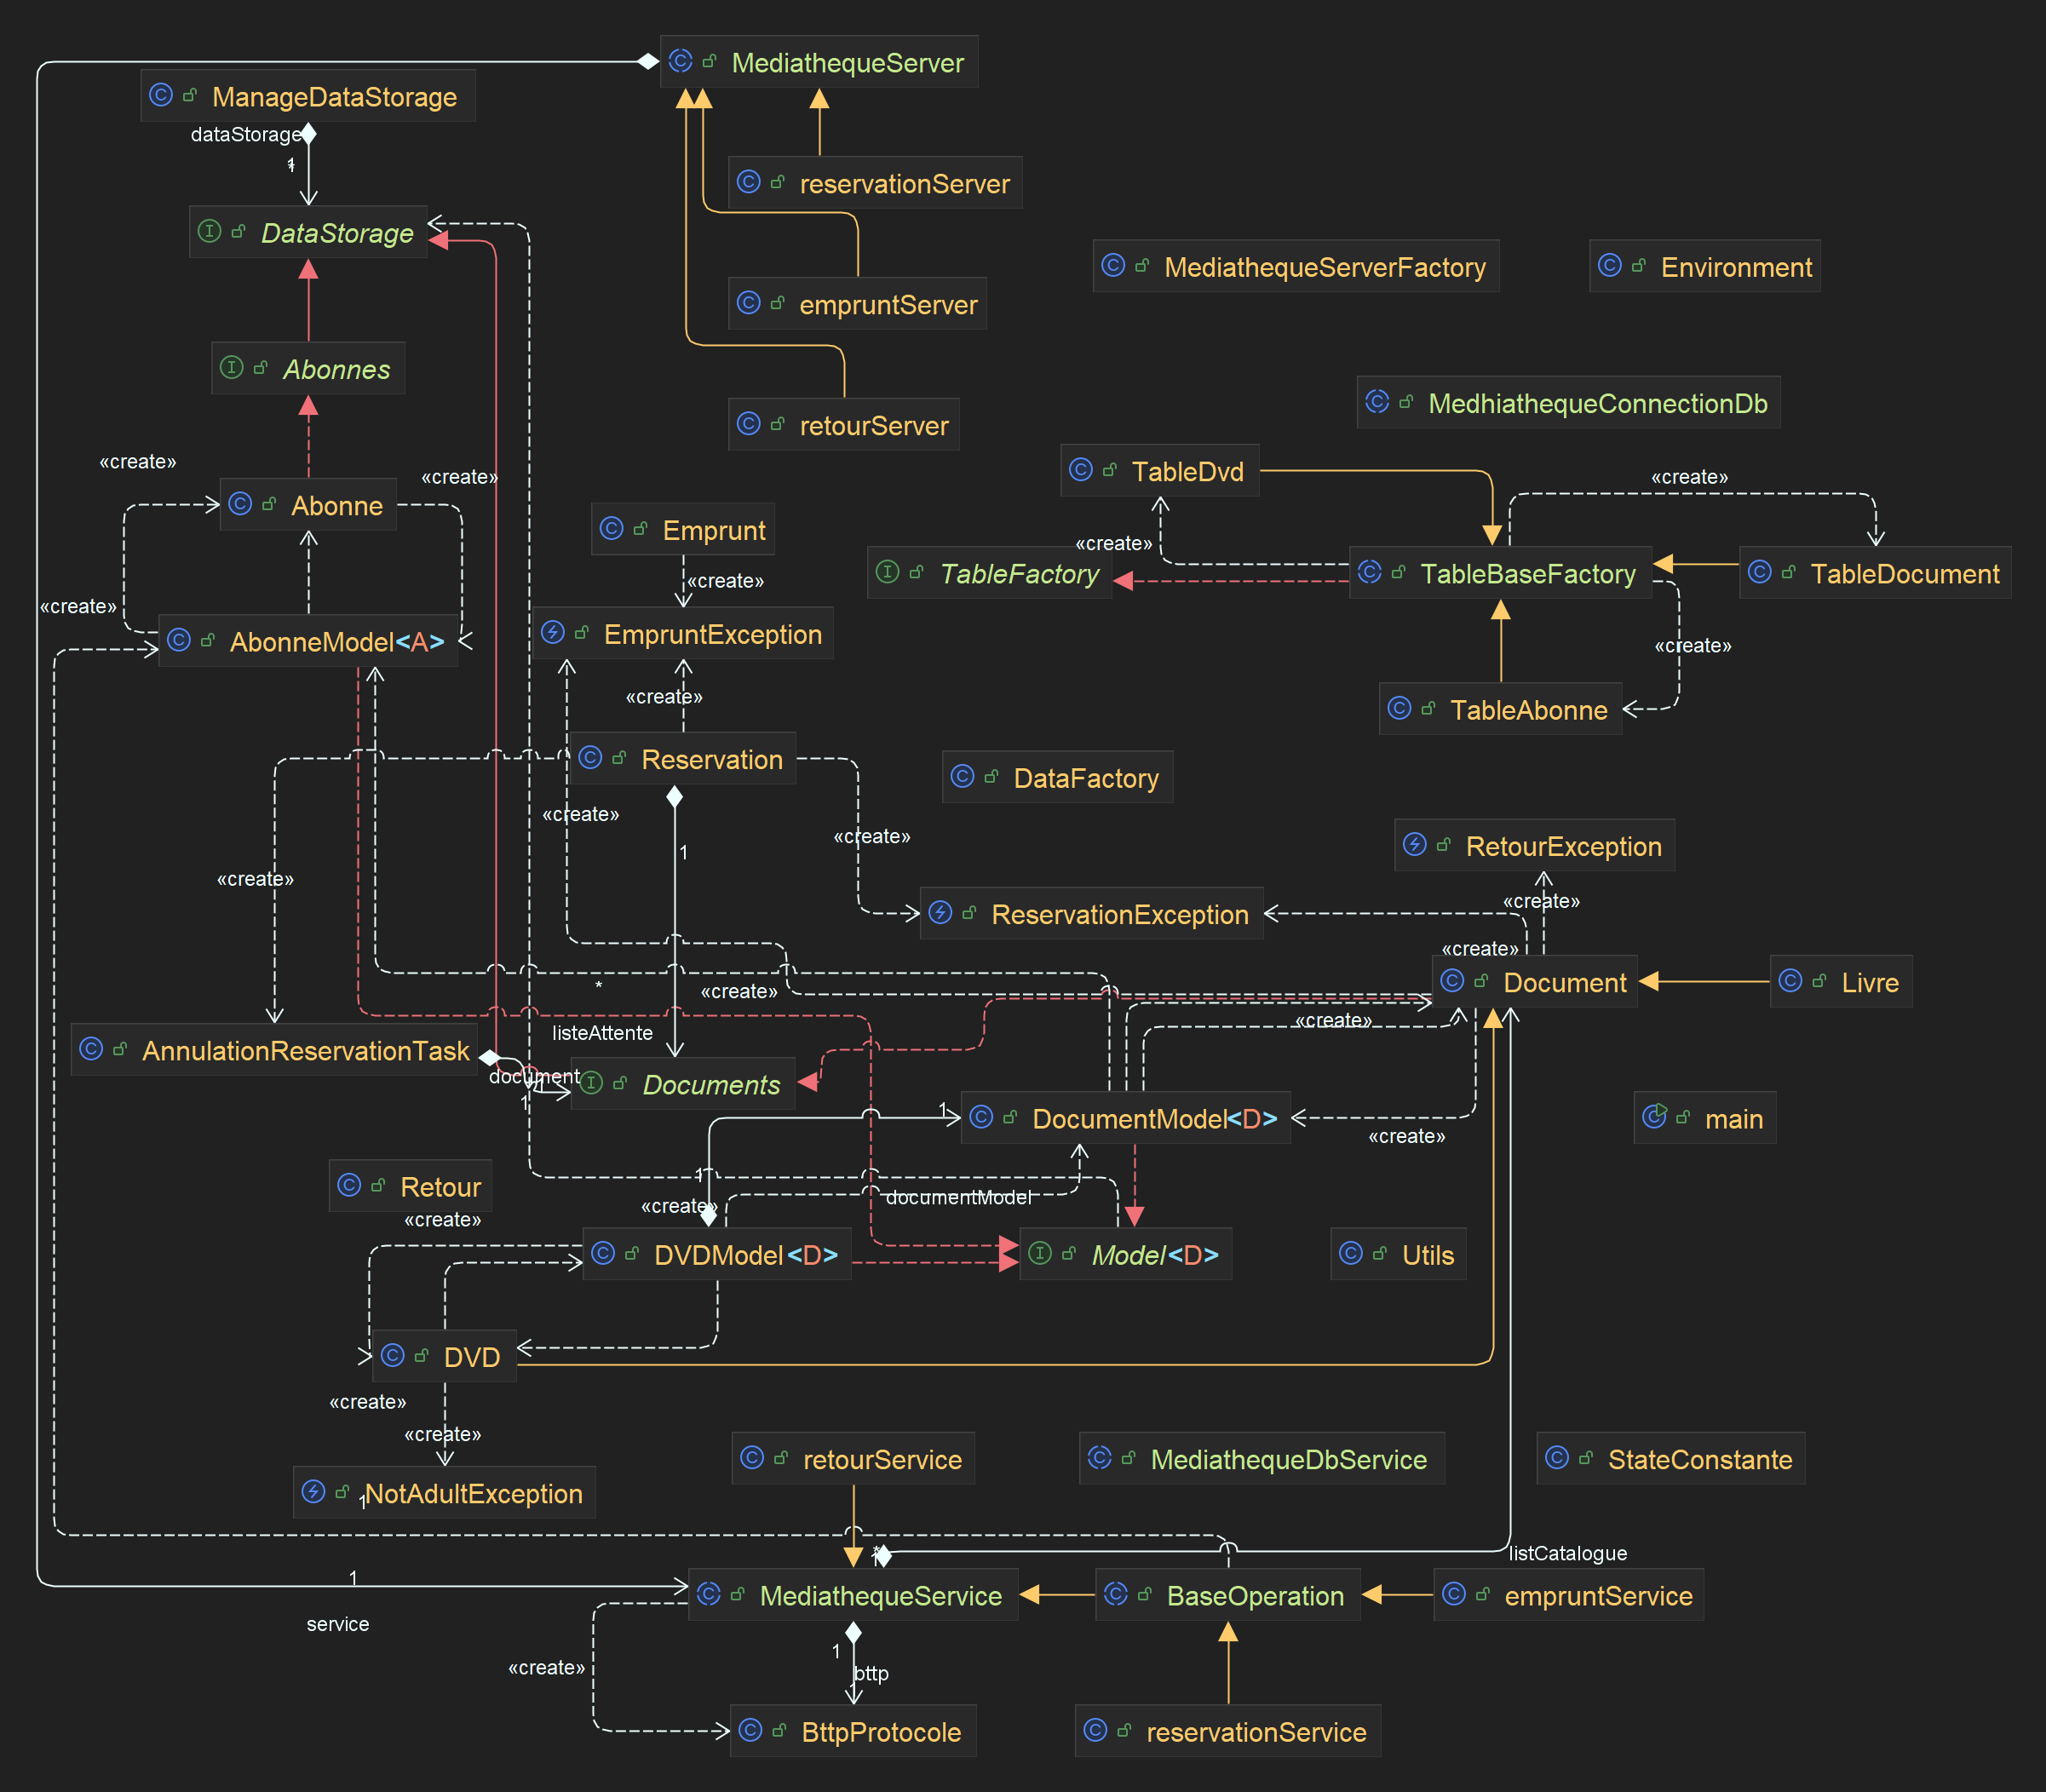
\includegraphics[width=1.1\textwidth]{image/uml5}
    \caption{Graphe de dépendance}
    \label{fig:dependency_graph}
\end{figure}


\section{Bibliothèques logicielles}

Nous avons utilisé plusieurs bibliothèques logicielles essentielles pour développer le projet. Voici les bibliothèques utilisées et leur utilisation spécifique :

\begin{itemize}
    \item \textbf{JDBC} : Cette bibliothèque a été utilisée pour interagir avec la base de données, permettant d'exécuter des requêtes SQL et de gérer les connexions conformément aux principes vus en cours.
    \item \textbf{Java .net} : Elle a été employée pour créer un protocole de communication via \textit{ServerSocket}, facilitant les échanges entre le client et le serveur.
    \item \textbf{Java .io} : Nous avons utilisé cette bibliothèque pour gérer les opérations d'entrée et de sortie, telles que la lecture et l'écriture de données ainsi que les exceptions associées.
    \item \textbf{Org .json} : Cette bibliothèque a été utilisée pour lire et traiter le fichier \textit{config.json}, ce qui nous permet de gérer les paramètres de configuration de manière sécurisée et flexible.
    \item \textbf{Java .util} : Nous avons largement utilisé cette bibliothèque pour manipuler différentes collections (\textit{Map}, \textit{List}), ainsi que pour les fonctionnalités de \textit{Scanner}, \textit{Date}, \textit{Timer} et \textit{TimerTask}. \textit{TimerTask} a été implémenté afin de limiter la durée maximale d'une réservation pour emprunter un document, évitant ainsi des réservations indéfinies.
    \item \textbf{Java .sql} : Cette bibliothèque a été intégrée pour permettre la communication en SQL avec la base de données, facilitant ainsi les opérations de création, lecture, mise à jour et suppression (CRUD) en utilisant également les exceptions spécifiques de cette bibliothèque.
\end{itemize}

L'utilisation de ces bibliothèques a permis de structurer notre application de manière efficace, en utilisant des outils et fonctionnalités standards de Java pour assurer maintenabilité et performance.

    \chapter{Échanges Client / Serveur}


\section{Client}

Pour la section client, nous avons établi plusieurs classes qui faciliteront la division du code en fichiers distincts.
Nous disposons donc d'un fichier dédié à la création de socket et au protocole BTTP, tandis qu'une autre classe permettra à l'utilisateur de choisir le service en fonction du port correspondant.


\section{Serveur}

Pour la gestion des entrées et des sorties de données, nous utilisons plusieurs classes :

\begin{itemize}
    \item \textbf{BufferedReader} : Utilisé pour lire les messages du client et du serveur.
    \item \textbf{PrintWriter} : Utilisé pour envoyer des messages dans le flux de sortie.
\end{itemize}


\section{Échanges Client / Serveur}

Le client se connecte au serveur en utilisant le protocole \textbf{BTTP}. Une fois connecté, le client et le serveur peuvent échanger des messages de manière synchrone. La connexion est initiée par le client en spécifiant l'adresse et le port du serveur. Les messages sont échangés en utilisant \texttt{BufferedReader} et \texttt{PrintWriter}. Le serveur traite les commandes reçues du client et renvoie les réponses appropriées.

Grâce à cette approche, une seule classe client est nécessaire, car la communication via BTTP permet une redirection efficace des ports vers le serveur souhaité pour chaque opération \textbf{(emprunt, réservation, retour)}. Le serveur dirige les requêtes vers les services appropriés, garantissant une gestion des différentes opérations possibles à l’heure actuelle et dans le futur.

Cette architecture permet une application performante et facile à maintenir, tout en permettant une extension future des fonctionnalités. Cette approche permet d'éviter la répétition de code en réinitialisant constamment les sockets, améliorant ainsi la performance et la maintenabilité de l'application. Nous avons fait une version basique du BTTP sans implémenter l’encodage/décodage, ce qui réduit le temps de communication mais diminue la sécurité.

    \chapter{Lien Application - Base de données}


\section{Modèle}

Concernant la liaison entre l’application et le serveur, nous avons utilisé \textbf{\textcolor{orange}{phpMyAdmin}} pour la gestion. Toute base de données MySQL peut quand même être utilisée étant donné que le SQL n’est pas standardisé pour tous les SGBD, ce qui s’assure que l’application soit fonctionnelle pour chaque utilisateur, à condition qu’ils utilisent le même SGBD que nous.

Nous avons mis en place des modèles pour représenter les tables de la base de données sous forme de classes. Cela nous permet de créer un \textbf{\textcolor{orange}{CRUD (Create, Read, Update, Delete)}} afin de réaliser différentes opérations sur la base de données. En outre, nous avons également développé une factory pour générer nos modèles de tables, garantissant ainsi que chaque membre de l’équipe dispose des mêmes modèles. De plus, pour chaque type de modèle, nous avons créé une interface pour rendre les classes flexibles et stables.

Lors de l’initialisation du projet, en exécutant la classe responsable de la création des tables, nous pouvons nous assurer que tous les membres du groupe disposent de la même architecture de base de données.


\section{Sauvegarde}

Pour gérer les différents états des documents, nous avons mis en place plusieurs types de structures pour stocker les documents en fonction de leur état. Par exemple, pour les documents réservés, nous les avons stockés dans une \texttt{HashMap} au sein de la classe effectuant l'opération (ex: Réservation), afin d'éviter de les regrouper tous dans une seule structure. Cette approche permet de localiser les documents selon leur état. Il est à noter que tous les documents retournés et donc libres sont stockés dans la structure principale lors de l'initialisation des services.

Lorsque nous fermons l’application correctement, nous nous assurons de stocker les données dans la base de données. Cette approche \textbf{minimise les échanges} avec la base de données car il s’agit d’une application \texttt{serverSocket} et non d’une application Web. Par conséquent, nous préférons stocker les données dans des variables ou tout autre structure de donnée pour interroger la base de données qu’au lancement et à la fermeture de l’application.

    \chapter{Concurrence}

Nous avons utilisé des blocs \texttt{synchronized} ainsi que des fonctions pour protéger les sections critiques de notre application, comme pour le paradigme du problème des philosophes afin d’assurer une exécution thread-safe. La concurrence se trouve entre les différentes opérations (réservation, retour, emprunt) car elles ne peuvent être exécutées simultanément sur un même document.

C’est en soi intuitif mais il est important de l’implémenter correctement pour éviter les conditions de course. Les sections synchronisées sont donc exécutées que lorsqu’elles sont disponibles, ceci garantit que l’application soit thread-safe.

    \chapter*{Maintenance évolutive}
\addcontentsline{toc}{chapter}{Maintenance évolutive}

\section{Ajout de nouveaux Documents}

\bigskip

L’ajout de nouveau Document nécessite d’implémenter l’interface correspondant aux Document ainsi que son
Modèle respectif si l'on veut le stocker dans la base de données.
La logique des opérations de Réservation, emprunt, retour ne changeront pas. C’est du \textbf{\textcolor{orange}{Pattern Bridge}} que nous nous sommes
inspirés pour implémenter les Documents.

\bigskip

\section{Passage en application web}

\bigskip

Pour passer sur une application Web nous devons revoir notre serveur de la médiathèque. Les opérations ne changeront pas mais
toute notre partie serveur devra être revu. Nous devons donc optimiser la maintenabilité de l’application afin de dissocier la médiathèque Server et son service du protocole de communication existant.

\bigskip

\section{Ajout nouveaux services}

\bigskip

La numérotation des ports ainsi que les urls sont géré par une class config qui lit un fichier config.json.
Nous avons utilisé ceci car c’est une bonne pratique en terme de sécurité de ne pas écrire en clair dans le code les urls port.

Donc, pour ajouter un nouveau service, il suffit d'attribuer les informations confidentielles à ce service dans la partie configuration, puis d'implémenter la classe du service. Il est important de ne pas oublierd'implémenter l'interface correspondante à la médiathèque, qui est propre à la relation entre le service et le serveur.


    \chapter{BretteSoft}

Pour la partie BretteSoft, nous avons implémenté une seule fonctionnalité : \textbf{Sitting Bull}.
Cette fonctionnalité permet de notifier un utilisateur par courriel lorsque ce dernier souhaite emprunter un document déjà réservé.


\section{Implémentation}

Pour implémenter cette fonctionnalité, nous avons intégré dans un fichier existant nommé \texttt{Utils} les fonctions nécessaires pour envoyer un courriel à une personne choisie, en l'occurrence le grand Wakan Tanka, à l'adresse suivante : \textbf{jean-francois.brette@u-paris.fr}. Cela signifie que lorsqu'une personne souhaite réserver un document, il lui sera demandé si elle souhaite être notifiée. Si elle répond positivement, un courriel lui sera envoyé dès que le document sera disponible.

\begin{itemize}
    \item \textbf{Javax.mail} : Bibliothèque utilisée pour envoyer des mails.
\end{itemize}

Concernant la sécurité, les paramètres du courriel, notamment l'adresse d'envoi, le port ainsi que le mot de passe, ont été stockés dans un fichier d'environnement.


\section{Processus}

Pour faire fonctionner cette bibliothèque, nous devons d'abord mettre en place certains éléments, notamment le mot de passe pour l'accès aux applications. En effet, pour pouvoir se connecter et ensuite envoyer un courriel à une personne, il est nécessaire de générer un mot de passe pour l'authentification. Auparavant, il suffisait de cocher une case dans la section "Less secure App" de Google, mais cette option a été supprimée depuis le 30 septembre 2024.

Sources :

\begin{itemize}
    \item \textbf{Envoyer mail SMTP} : \href{https://kb.synology.com/fr-fr/SRM/tutorial/How_to_use_Gmail_SMTP_server_to_send_emails_for_SRM}{Gmail SMTP server to send emails for SRM}
    \item \textbf{Less secure App} : \href{https://support.google.com/accounts/answer/6010255?sjid=6174101903992956370-EU}{Google Accounts Answer}
\end{itemize}


\section{Alternatives d'implémentation}

Il existe différentes manières d'implémenter la fonctionnalité BretteSoft.
Par exemple, nous aurions pu :

\begin{itemize}
    \item Créer notre propre serveur SMTP pour envoyer les messages.
    \item Utiliser d'autres bibliothèques ou services proposant l'envoie de mail.
\end{itemize}

Cependant, pour des raisons de sécurité et de simplicité, nous avons préféré utiliser un service déjà existant comme Javax.mail.
Et d'utiliser le serveur SMTP de Gmail pour envoyer les mails car c'est un service déjà utilisé en entreprise.



\end{document}
